%%%%%%%%%%%%%%%%%%%%%%%%%%%%%%%%%%%%%%%%%
% University/School Laboratory Report
% LaTeX Template
% Version 3.0 (4/2/13)
%
% This template has been downloaded from:
% http://www.LaTeXTemplates.com
%
% Original author:
% Linux and Unix Users Group at Virginia Tech Wiki 
% (https://vtluug.org/wiki/Example_LaTeX_chem_lab_report)
%
% License:
% CC BY-NC-SA 3.0 (http://creativecommons.org/licenses/by-nc-sa/3.0/)
%
%%%%%%%%%%%%%%%%%%%%%%%%%%%%%%%%%%%%%%%%%

%----------------------------------------------------------------------------------------
%	PACKAGES AND DOCUMENT CONFIGURATIONS
%----------------------------------------------------------------------------------------

\documentclass{article}

\usepackage[version=3]{mhchem} % Package for chemical equation typesetting
\usepackage{siunitx} % Provides the \SI{}{} command for typesetting SI units

\usepackage[top=1in, bottom=1in, right=1in, left=1in]{geometry}

%Add code formating
\usepackage{listings}
\lstset{tabsize=2}

\usepackage{hyperref}

\usepackage{amssymb}

\usepackage{enumerate}

%Add extra support for image placement
\usepackage{float}

\usepackage{mcode}

\usepackage{graphicx} % Required for the inclusion of images

\setlength\parindent{0pt} % Removes all indentation from paragraphs

\renewcommand{\labelenumi}{\alph{enumi}.} % Make numbering in the enumerate environment by letter rather than number (e.g. section 6)

%\usepackage{times} % Uncomment to use the Times New Roman font

%----------------------------------------------------------------------------------------
%	DOCUMENT INFORMATION
%----------------------------------------------------------------------------------------

\title{Keysight Hacking Platform Getting Started} % Title

\author{Blake \textsc{Vermeer}} % Author name

\date{\today} % Date for the report

\begin{document}

\maketitle % Insert the title, author and date

\begin{center}
\begin{tabular}{l r}
Date Performed: & March 21, 2017 \\ % Date the experiment was performed
Company: & Keysight Technologies % Company
\end{tabular}
\end{center}

% If you wish to include an abstract, uncomment the lines below
% \begin{abstract}
% Abstract text
% \end{abstract}

%----------------------------------------------------------------------------------------
%	OVERVIEW
%----------------------------------------------------------------------------------------
\section{Overview}

The Keysight Hacking Platform is designed to have a development workflow similar to how firmware is developed in most Keysight products while yet at the same time being flexible enough that students can develop their own software / hardware for a Hackathon. \\

The Keysight Hacking Platform consists of:

	\begin{itemize}
		
		\item Raspberry Pi 3 with 2.8" capacitive touch screen shield
		
		\item Custom Yocto Linux image pre-loaded on the Raspberry Pi 3
		
		\item Fedora Linux Virtual Machine image with Qt Creator and the Yocto SDK pre-installed and configured with Qt Creator
		
	\end{itemize}

The general workflow for creating applications using the KHP is the application is created in the Qt Creator program that is pre-installed in the virtual machine image. The application is then cross-compiled by Qt Creator using the Yocto SDK and is then sent over WiFi to the Raspberry Pi where the application is run and can be debugged remotely using Qt Creator.

	\begin{figure}[H]
		\centering
		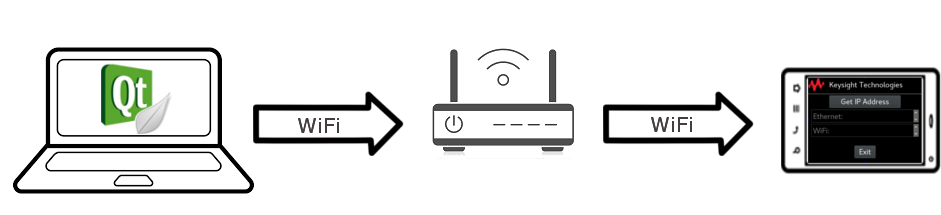
\includegraphics[scale=0.5]{pics/Deployment_Workflow.png}
		\caption{Qt App Deployment Workflow}
		\label{Qt_App_Deployment}
	\end{figure}



%----------------------------------------------------------------------------------------
%	Installing VirtualBox
%----------------------------------------------------------------------------------------
\section{Installing VirtualBox}




%----------------------------------------------------------------------------------------
%	Importing the Virtual Machine
%----------------------------------------------------------------------------------------
\section{Import the Virtual Machine}

After install VirtualBox, the next step is to import the virtual machine image into VirtualBox. After starting up VirtualBox, choose "Import Appliance..." from the file menu.

	\begin{figure}[H]
		\centering
		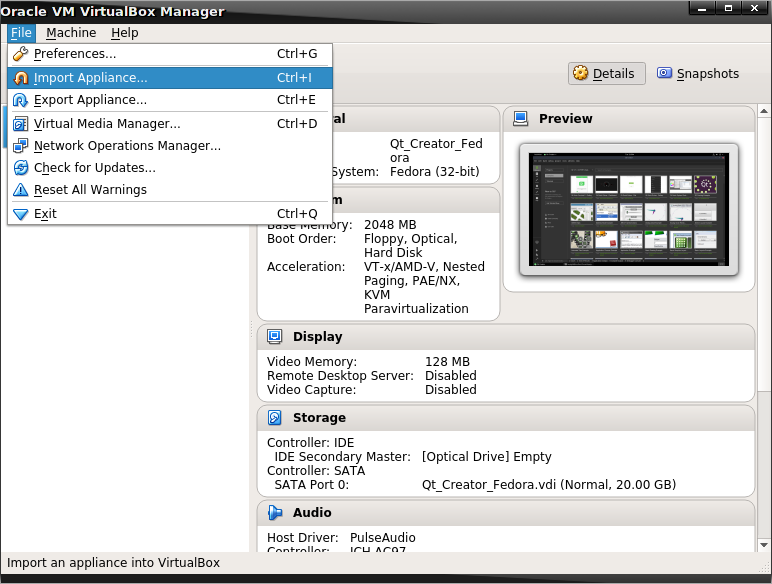
\includegraphics[scale=0.35]{pics/VirtualBox_Import_Appliance.png}
		\caption{Import Virtual Machine}
		\label{Import_Virtual_Machine}
	\end{figure}


Navigate to the location of the virtual machine image (Qt\_Creator\_Fedora.ova) and then click next. In the next screen that appears (Appliance settings) make sure to click the checkbox to reinitialize the MAC addresses of all the network cards.


	\begin{figure}[H]
		\centering
		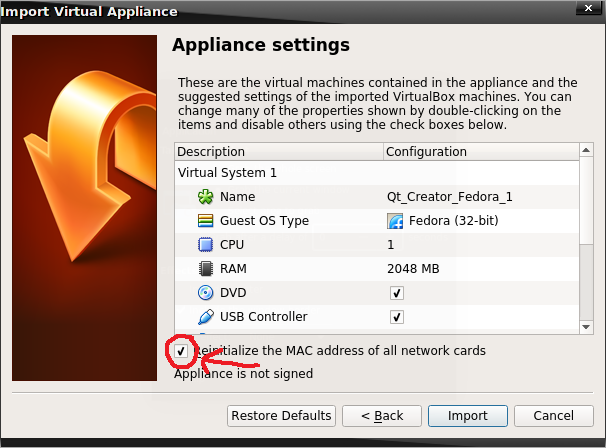
\includegraphics[scale=0.75]{pics/VirtualBox_Appliance_Settings.png}
		\caption{Import Virtual Machine Settings}
		\label{Import_Virtual_Machine_Settings}
	\end{figure}

After importing the virtual machine image, the main VirtualBox screen should appear similar to Figure \ref{VirtualBox_Main_Window}. To start the virtual machine, highlight the "Qt\_Creator\_Fedora" virtual machine from the list and then click the start button.

	\begin{figure}[H]
		\centering
		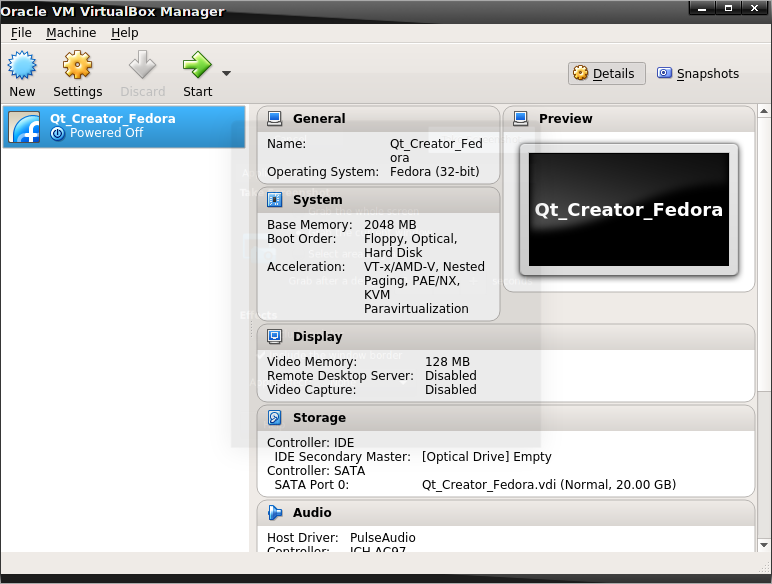
\includegraphics[scale=0.35]{pics/VirtualBox_Main_View.png}
		\caption{VirtualBox Main Window}
		\label{VirtualBox_Main_Window}
	\end{figure}


%----------------------------------------------------------------------------------------
%	Launching the Virtual Machine
%----------------------------------------------------------------------------------------
\section{Launching the Virtual Machine}




%----------------------------------------------------------------------------------------
%	Start Qt Creator and Connect to the Raspberry Pi
%----------------------------------------------------------------------------------------
\section{Start Qt Creator and Connect to the Raspberry Pi}




%----------------------------------------------------------------------------------------
%	APPENDIX
%----------------------------------------------------------------------------------------

%\newpage
%\section{Appendix}

%\begin{enumerate}

	
%	\item[1. a.)] \lstinputlisting{../MATLAB/problem_1a.m}
	

%\end{enumerate}






%----------------------------------------------------------------------------------------


\end{document}